% Knowledge Graph Ontology — Schema Diagram
% Compile with: pdflatex knowledge-graph-ontology.tex
\documentclass[border=14pt]{standalone}

\usepackage[T1]{fontenc}
\usepackage[english]{babel}
\usepackage{lmodern}
\usepackage{amsmath}
\usepackage{xcolor}
\usepackage{tikz}
\usetikzlibrary{
    decorations.pathmorphing,
    decorations.pathreplacing,
    arrows.meta,
    positioning,
    calc,
    shapes.geometric,
    backgrounds,
    fit
}

%% ---------- Colour palette ----------
\definecolor{ink}        {HTML}{1F2433}
\definecolor{soft}       {HTML}{9CA3AF}
\definecolor{accent}     {HTML}{3A6E5B}
\definecolor{accentbg}   {HTML}{E4EFE9}

%% --- entity-type colours (matched to distillation pipeline lenses) ---
\definecolor{c1}{HTML}{4A6FA5}\definecolor{c1bg}{HTML}{EBF1F9}  % Topic
\definecolor{c2}{HTML}{C9883A}\definecolor{c2bg}{HTML}{FBF2DD}  % Author
\definecolor{c3}{HTML}{B85C92}\definecolor{c3bg}{HTML}{F8E8F0}  % Assumption
\definecolor{c4}{HTML}{4F8A6B}\definecolor{c4bg}{HTML}{E7F0EA}  % Theory
\definecolor{c5}{HTML}{C8553D}\definecolor{c5bg}{HTML}{FBEBE6}  % Conclusion
\definecolor{c6}{HTML}{5B6E8C}\definecolor{c6bg}{HTML}{ECEFF4}  % Methodology

\definecolor{kgbg}       {HTML}{FBFCFE}
\definecolor{kgborder}   {HTML}{C8CFDB}

\begin{document}
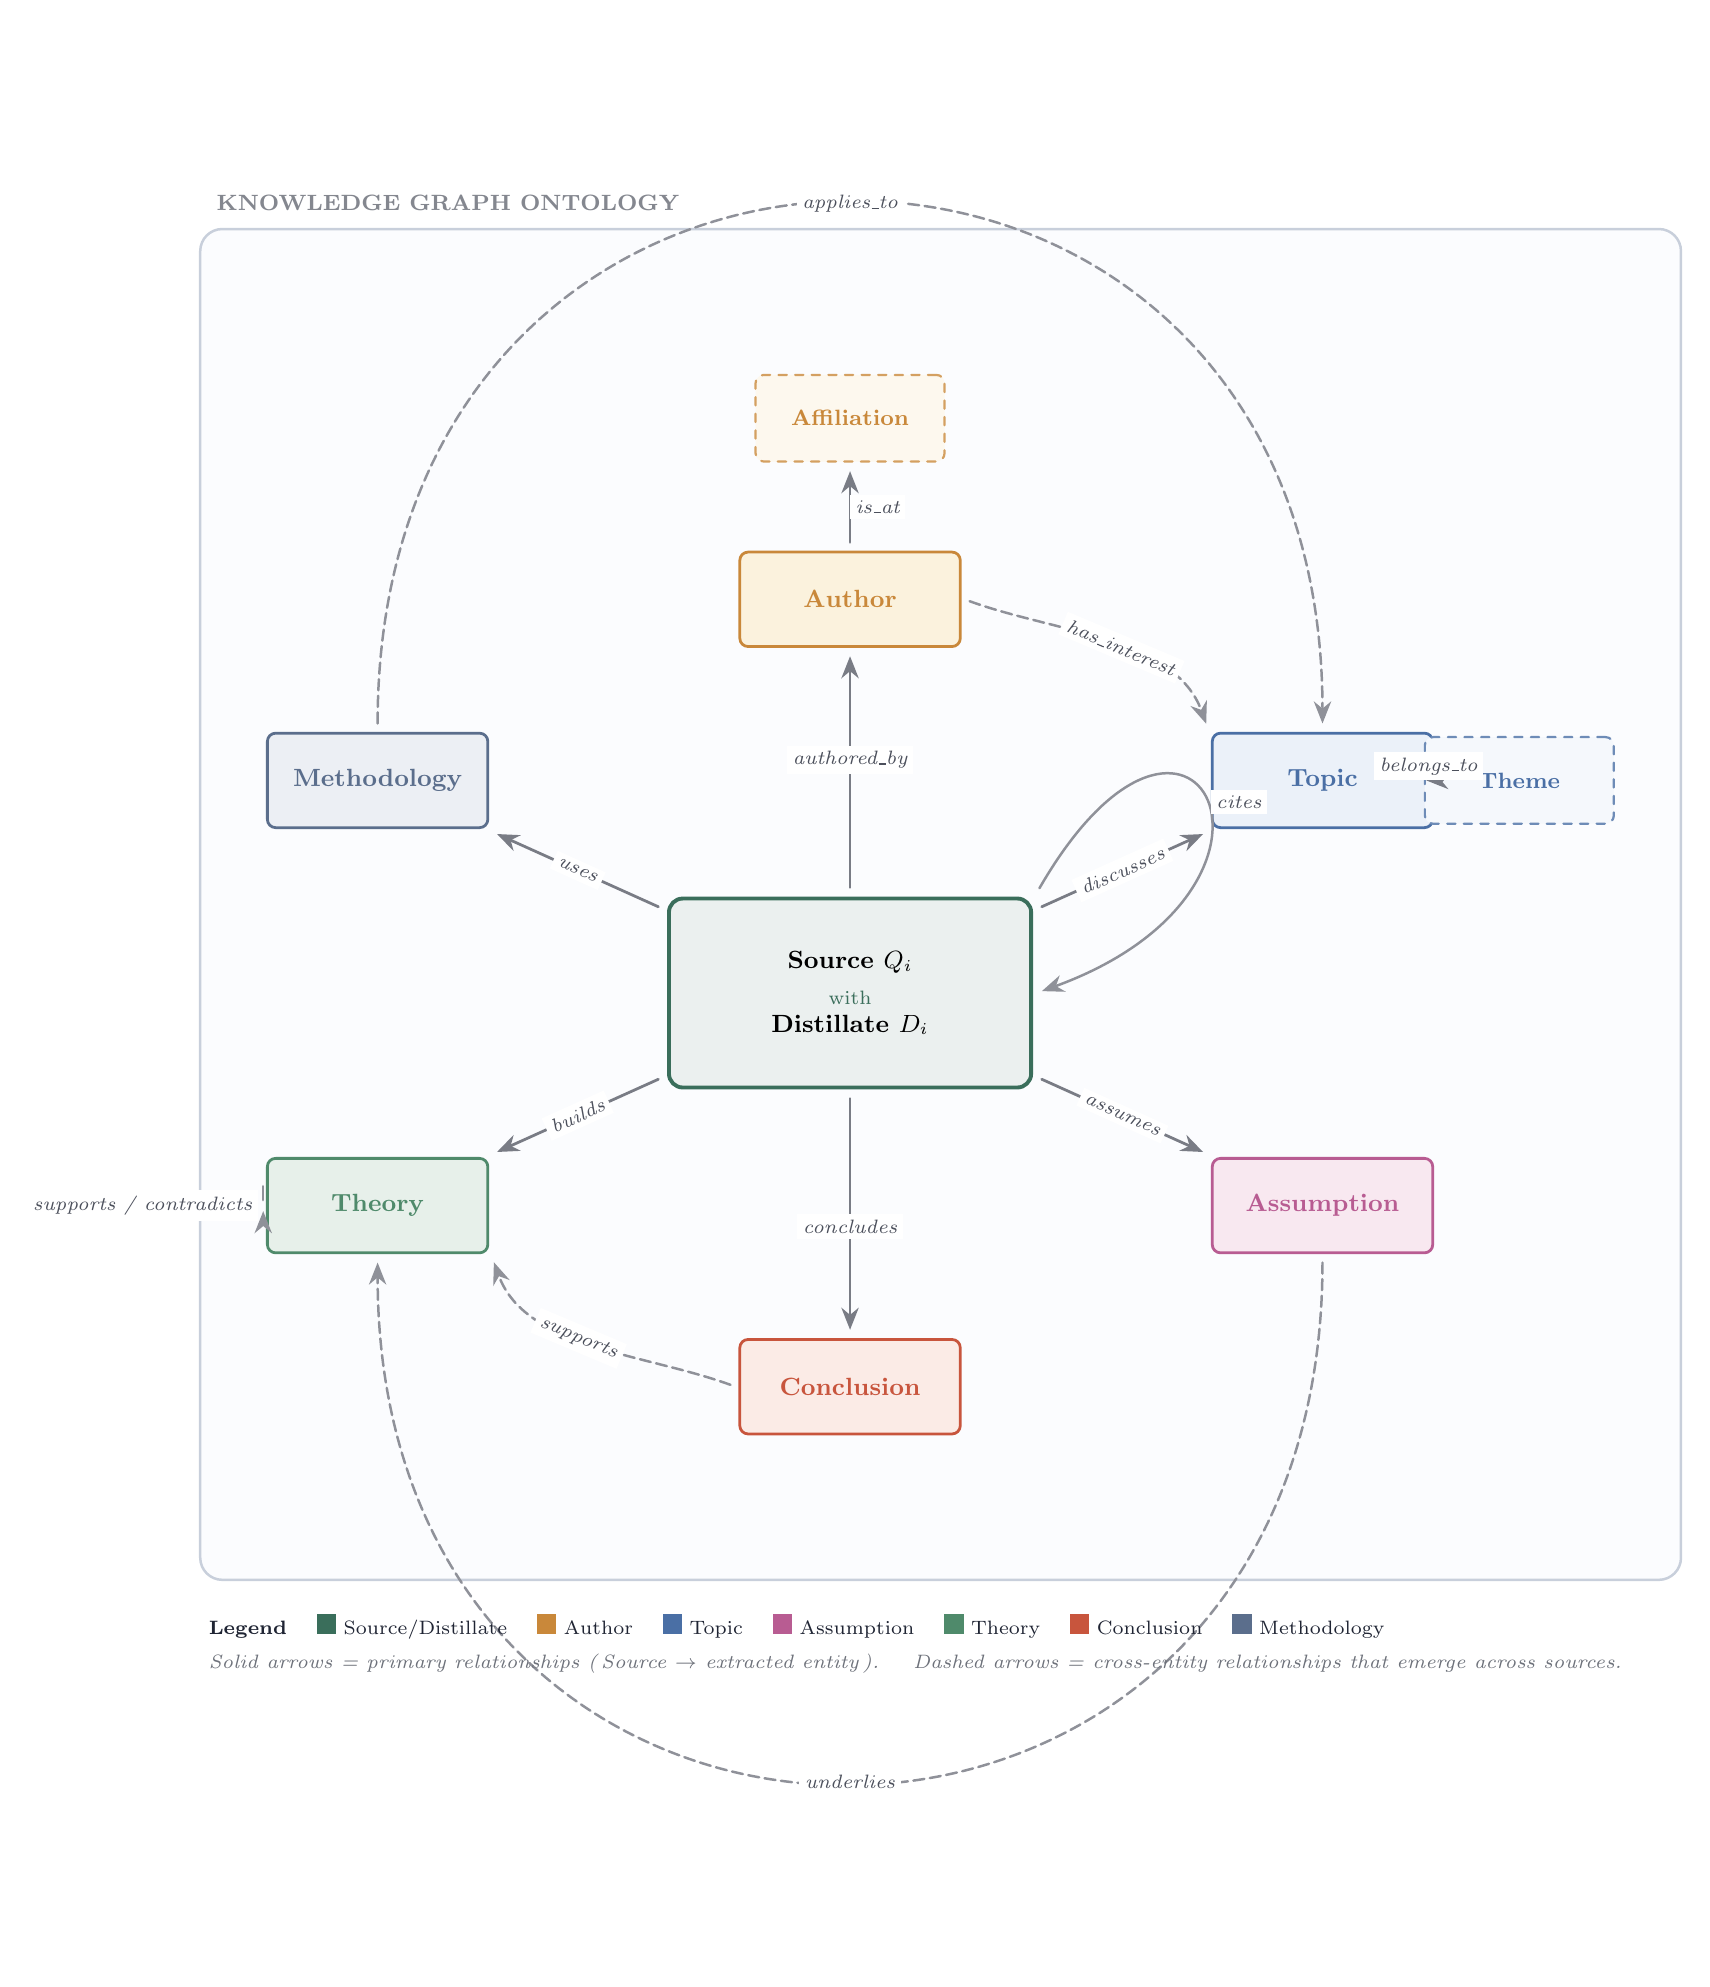
\begin{tikzpicture}[
    line cap=round, line join=round,
    >={Stealth[length=2.8mm, width=2.2mm]},
    %% --- semantic styles ---
    entity/.style       = {rectangle, line width=1pt, rounded corners=3pt,
                           minimum width=28mm, minimum height=12mm,
                           font=\small\bfseries, align=center,
                           inner sep=4pt, outer sep=1.5pt},
    centerentity/.style = {rectangle, draw=accent, fill=accent!10,
                           line width=1.4pt, rounded corners=5pt,
                           minimum width=46mm, minimum height=24mm,
                           font=\small\bfseries, align=center,
                           inner sep=6pt, outer sep=2pt},
    secondary/.style    = {rectangle, line width=0.8pt, rounded corners=3pt,
                           minimum width=24mm, minimum height=11mm,
                           font=\footnotesize\bfseries, align=center,
                           inner sep=3pt, dashed, outer sep=1.5pt},
    primaryedge/.style  = {->, draw=ink!60, line width=1pt,
                           shorten >=2pt, shorten <=2pt},
    crossedge/.style    = {->, draw=ink!50, line width=0.9pt,
                           shorten >=2pt, shorten <=2pt,
                           dash pattern=on 4pt off 2pt},
    selfedge/.style     = {->, draw=ink!50, line width=0.9pt,
                           shorten >=2pt, shorten <=2pt},
    edgelabel/.style    = {font=\scriptsize\itshape, text=ink!80,
                           fill=white, inner sep=2pt, outer sep=0pt},
    sectionlabel/.style = {font=\footnotesize\bfseries, text=ink!55}
]

%% ============================================================
%% CENTER — Source + Distillate
%% ============================================================
\node[centerentity] (S) at (0, 0) {%
    Source $Q_i$\\[2pt]
    {\scriptsize\mdseries\color{accent} with}\\[-1pt]
    Distillate $D_i$
};

%% ============================================================
%% PRIMARY ENTITIES — 6 dimensions, large radial layout
%% ============================================================
\node[entity, fill=c2bg, draw=c2, text=c2] (Author)       at (0,    5.0)  {Author};
\node[entity, fill=c1bg, draw=c1, text=c1] (Topic)        at (6.0,  2.7)  {Topic};
\node[entity, fill=c3bg, draw=c3, text=c3] (Assumption)   at (6.0, -2.7)  {Assumption};
\node[entity, fill=c5bg, draw=c5, text=c5] (Conclusion)   at (0,   -5.0)  {Conclusion};
\node[entity, fill=c4bg, draw=c4, text=c4] (Theory)       at (-6.0,-2.7)  {Theory};
\node[entity, fill=c6bg, draw=c6, text=c6] (Methodology)  at (-6.0, 2.7)  {Methodology};

%% ============================================================
%% SECONDARY ENTITIES — pushed outward, clear of the cross-arcs
%% ============================================================
\node[secondary, fill=c2bg!50, draw=c2!80, text=c2]
    (Affil) at (0,   7.3) {Affiliation};
\node[secondary, fill=c1bg!50, draw=c1!80, text=c1]
    (Theme) at (8.5, 2.7) {Theme};

%% ============================================================
%% PRIMARY EDGES — radial spokes from Source
%% ============================================================
\draw[primaryedge] (S) -- node[edgelabel, pos=0.55]
    {authored\_by} (Author);
\draw[primaryedge] (S) -- node[edgelabel, pos=0.5, sloped]
    {discusses}   (Topic);
\draw[primaryedge] (S) -- node[edgelabel, pos=0.5, sloped]
    {assumes}     (Assumption);
\draw[primaryedge] (S) -- node[edgelabel, pos=0.55]
    {concludes}   (Conclusion);
\draw[primaryedge] (S) -- node[edgelabel, pos=0.5, sloped]
    {builds}      (Theory);
\draw[primaryedge] (S) -- node[edgelabel, pos=0.5, sloped]
    {uses}        (Methodology);

%% ============================================================
%% SECONDARY EDGES — to grouping entities
%% ============================================================
\draw[primaryedge] (Author) -- node[edgelabel, right] {is\_at}      (Affil);
\draw[primaryedge] (Topic)  -- node[edgelabel, above] {belongs\_to} (Theme);

%% ============================================================
%% CROSS-ENTITY EDGES — outer arcs only (no centre crossings)
%% ============================================================
% Author --has_interest--> Topic   (short arc, upper-right outside corner)
\draw[crossedge] (Author.east) to[out=-20, in=110, looseness=0.9]
    node[edgelabel, sloped, pos=0.55] {has\_interest}
    (Topic.north west);

% Methodology --applies_to--> Topic   (long arc OVER the top, above Affiliation)
\draw[crossedge] (Methodology.north) to[out=90, in=90, looseness=1.9]
    node[edgelabel, pos=0.5] {applies\_to}
    (Topic.north);

% Conclusion --supports--> Theory   (short arc, lower-left outside corner)
\draw[crossedge] (Conclusion.west) to[out=160, in=-70, looseness=0.9]
    node[edgelabel, sloped, pos=0.55] {supports}
    (Theory.south east);

% Assumption --underlies--> Theory   (long arc UNDER the bottom)
\draw[crossedge] (Assumption.south) to[out=-90, in=-90, looseness=1.9]
    node[edgelabel, pos=0.5] {underlies}
    (Theory.south);

%% ============================================================
%% SELF-LOOPS
%% ============================================================
% Theory: supports / contradicts  (loop on the left side, well clear)
\draw[selfedge] (Theory.west) to[out=160, in=200, looseness=10]
    node[edgelabel, anchor=east, xshift=-2pt] {supports / contradicts}
    (Theory.west);

% Source: cites  (compact loop inside the centre, north-east corner)
\draw[selfedge] (S.north east) to[out=60, in=20, looseness=8]
    node[edgelabel, anchor=west, xshift=2pt] {cites}
    (S.east);

%% ============================================================
%% Background container — generous padding for the outer arcs
%% ============================================================
\begin{scope}[on background layer]
    \node[draw=kgborder, fill=kgbg, rounded corners=8pt,
          line width=0.9pt,
          inner xsep=8mm, inner ysep=18mm,
          fit=(Author) (Topic) (Assumption) (Conclusion) (Theory)
              (Methodology) (Affil) (Theme) (S)] (KGBOX) {};
\end{scope}

\node[sectionlabel, anchor=south west]
    at ($(KGBOX.north west) + (1mm, 1mm)$) {KNOWLEDGE GRAPH ONTOLOGY};

%% ============================================================
%% Legend
%% ============================================================
\node[anchor=north west, font=\scriptsize, text=ink]
    at ($(KGBOX.south west) + (0, -3mm)$)
    {\textbf{Legend} \quad
     \textcolor{accent}{\rule{2.5mm}{2.5mm}}~Source/Distillate \quad
     \textcolor{c2}{\rule{2.5mm}{2.5mm}}~Author \quad
     \textcolor{c1}{\rule{2.5mm}{2.5mm}}~Topic \quad
     \textcolor{c3}{\rule{2.5mm}{2.5mm}}~Assumption \quad
     \textcolor{c4}{\rule{2.5mm}{2.5mm}}~Theory \quad
     \textcolor{c5}{\rule{2.5mm}{2.5mm}}~Conclusion \quad
     \textcolor{c6}{\rule{2.5mm}{2.5mm}}~Methodology};

\node[anchor=north west, font=\scriptsize\itshape, text=ink!65]
    at ($(KGBOX.south west) + (0, -8mm)$)
    {Solid arrows = primary relationships (\,Source $\to$ extracted entity\,). \quad
     Dashed arrows = cross-entity relationships that emerge across sources.};

\end{tikzpicture}
\end{document}
